\likechapter{Вступ}

У даній роботі були досліджені 3 зразки чотирьохполюсників, та знайдена їх амплітудно-частотна та фазо-частотна характеристика. Оскільки вся інформація, що залишилася у авторів, зводиться до аж однієї, хоч і красивої, але все ж таки однієї фотографії жертв насильства \ref{photo}, побудувати детальні теоретичні моделі неможливо. Для проведення даної роботи ми використовували один дивовижний осцилограф моделі TDS2024C та якийсь там функціональний генератор.

Оскільки дана робота надзвичайно схожа на №2, яку ми також виконували, то цей звіт написаний у не сильно розгорнутому стилі. \sout{Ну а що писати коли і так все всім ясно}

\begin{figure}[h]
\center{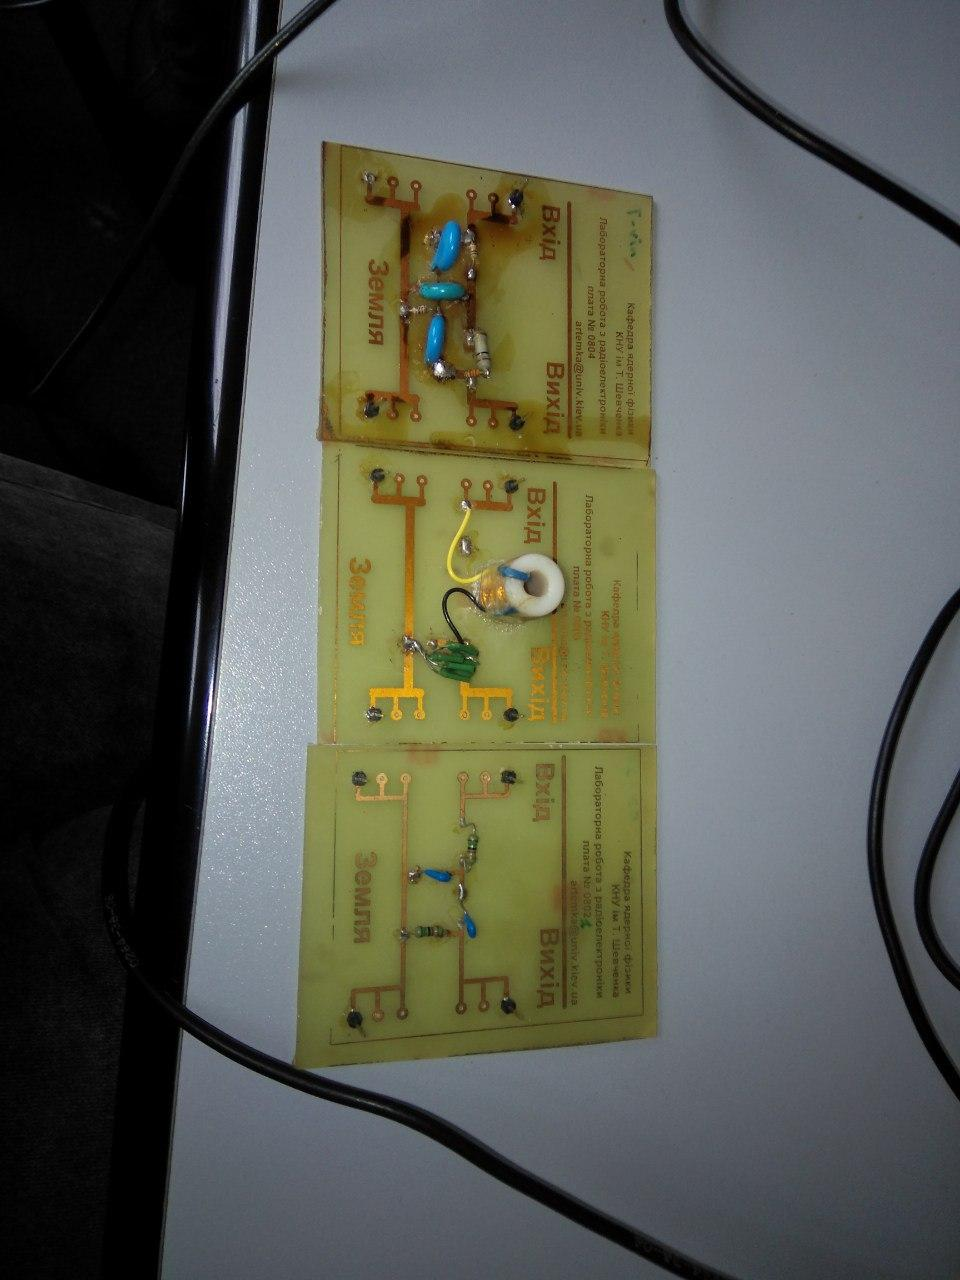
\includegraphics[width=0.9\linewidth]{img/photo}}
\caption{Жертви насильства. Нумерація у роботі: від 1 до 3, зліва направо.}
\label{photo}
\end{figure}